\section{LDOS 1D}

\subsection{First problem}

\begin{figure}[H]
    \centering    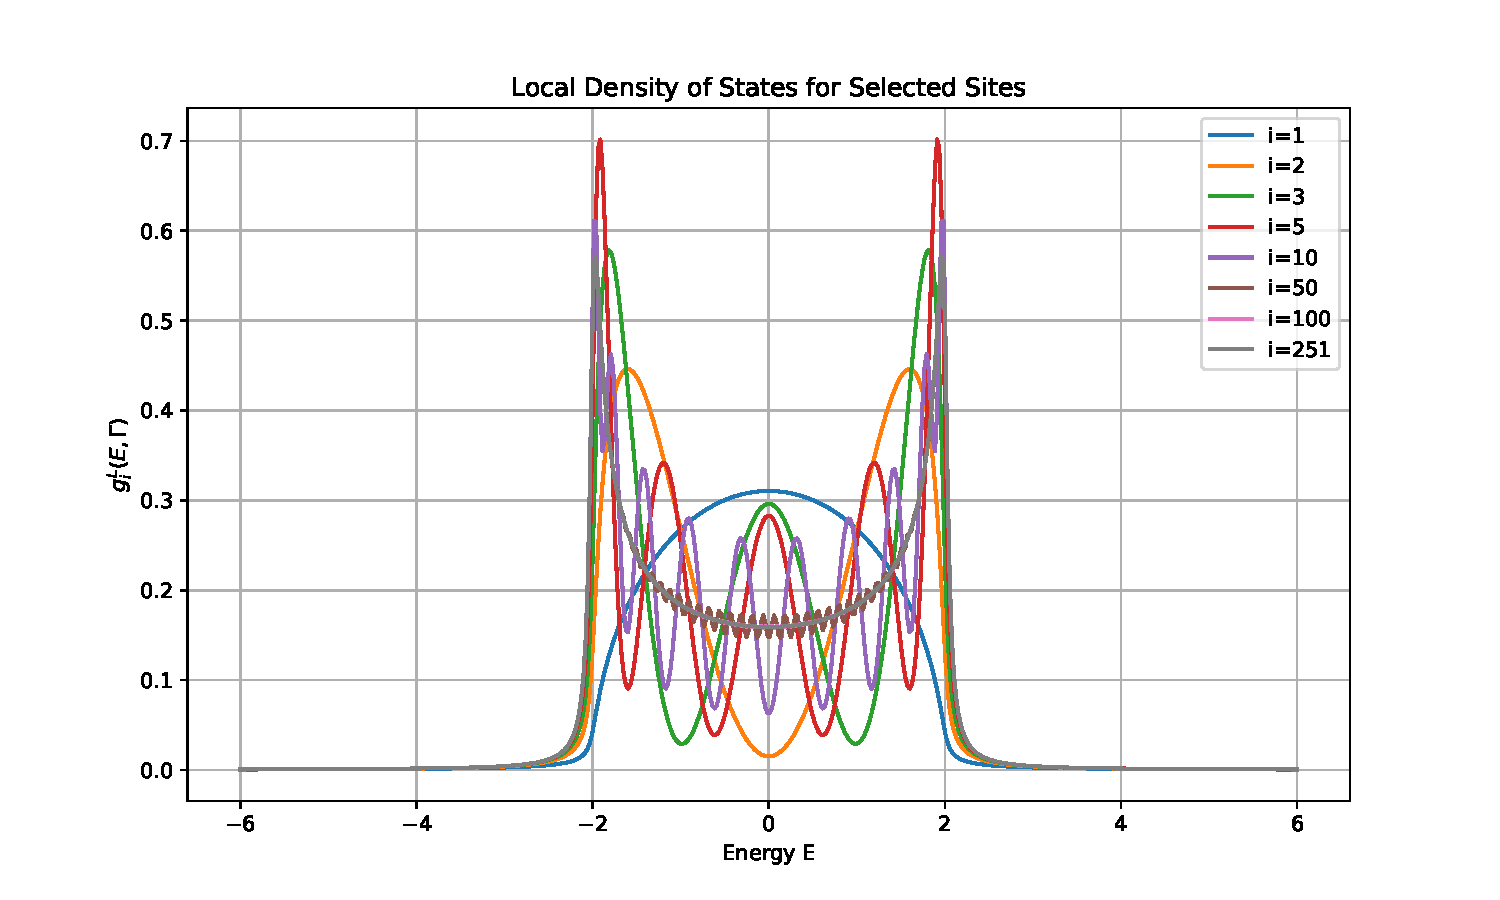
\includegraphics[width=\textwidth]{Figures/task1.pdf}
    \caption{Local density of states plotted for a 1D chain of length $N=501$. The index $i$ corresponds to the site number in the chain.}
    \label{fig:task1}
\end{figure}
Noticeable in Fig. \ref{fig:task1} is that the LDOS is symmetric around the central energy. For increasing $i$ the number of nodes in the LDOS oscillation increases. The central amplitude also decreases while the amplitude at $E = \pm 2$ increases.